\chapter{Schrittl"angensteuerung\label{chapter:schrittlaenge}}
\lhead{Schrittl"angensteuerung}
\begin{refsection}
\chapterauthor{Pascal Horat und Matthias Kn"opfel}


\section{Problemstellung}
\rhead{Problemstellung}

Mit den numerischen Verfahren wird die L"osung schrittweise konstruiert, was bei \glqq engen Kurven\grqq~zu Problemen f"uhren kann.
Im schlimmsten Fall verpasst die L"osung die Kurve ganz.
Wenn man aber immer nur ganz kleine Schritte macht, dauert die Berechnung der L"osung sehr lange, vor allem auf \glqq geraden Strecken\grqq~wird unn"otig Rechenzeit verschwendet.

M"ogliche Fragestellungen: mit welchen Kriterien steuert man die Anpassung der Schrittl"ange?
Wie "andert sich die Genauigkeit der L"osung?
Weniger unn"otige Rechenschritte reduzieren auch die Gefahr von Rundungsfehlern, die das Resultat verf"alschen k"onnen, kann man diesen Effekt messen?
Wie kann man den Tradeoff zwischen Rechenaufwand und Genauigkeit beziffern oder visualisieren?


\section{Beispiel}
\rhead{Beispiel}

Um die Schrittl"angenproblematik zu erl"autern, wird ein geeignetes Beispiel ben"otigt, welches folgende Anforderung erf"ullt: 
\begin{itemize}
\item Die L"osung sollte \glqq lange gerade Strecken\grqq~und Stellen mit grossen "Anderungen beinhalten, damit die Algorithmen an ihre Grenzen kommen.
\item Das Problem sollte schnell und leicht verst"andlich sein, denn in diesem Kapitel geht es schliesslich um die Schrittl"angensteuerung.
\item Das Konzept der Schrittl"angensteuerung und dessen Vorteile sollten damit auf einfache Weise visualisiert werden k"onnen.
\end{itemize}
Auf Grund diesen Voraussetzungen wurde als Beispielproblem das allgemein bekannte \em Zweik"orperproblem\em~gew"ahlt.
Bei diesem Problem geht es darum, das Verhalten zweier K"orper, welche ohne "aussere Einflüsse miteinander wechselwirken, zu berechnen. 
Die Berechnungen werden zur Vereinfachung nach den Gesetzen und Axiomen von Newton vorgenommen, das heisst die relativistischen Effekte gem"ass Einstein werden ausser Acht gelassen.
Ausserdem wird von Massepunkten ausgegangen.
Damit gilt nach dem Newtonschen Gravitionsgesetz folgende Gleichung:
\begin{equation} \label{eq:newton}
F_1 = F_2=\frac{G m_1 m_2}{r^2}
\end{equation}
In obiger Formel ist $G$ die universelle Gravitationskonstante und $r$ der Abstand zwischen den beiden Massenpunkten.
Eine weitere Vereinfachung bringt die Annahme, dass beide Massen gleich sind. 
Damit erfahren beide K"orper vom Betrag her die selbe Momentanbeschleunigung $a$.
\begin{equation}
F=\frac{G m^2}{r^2}=m a
\end{equation}
Auf die momentane Beschleunigung umgeformt gilt somit:
\begin{equation}
a=\frac{G m}{r^2} \label{eq:beschleunigungSkalar}
\end{equation}
F"ur die weitere Betrachtung ist es sinnvoll in mehreren Dimensionen zu rechnen.
Aus diesem Grund erfährt die Formel nun ein Upgrade zur Vektorrechnung.
Jeder K"orper $k$ hat eine bestimmte Position welche durch seinen Ortsvektor $\vec{s_k}$ beschrieben wird.
Der Abstand zwischen zwei K"orpern $K_1$ und $K_2$ ist damit die Differenz der beiden Ortsvektoren  $\vec{s_1}$ und $\vec{s_2}$:
\begin{equation} \label{eq:abstand}
\vec{r_{12}}= \vec{s_2}-\vec{s_1}
\end{equation}
Die Gleichung (\ref{eq:beschleunigungSkalar}) sieht in Vektorschreibweise umgeformt also folgendermassen aus:
\begin{equation} \label{eq:gravitationVektor}
\vec{a_1} =\frac{G m}{\mid \vec{r_{12}}\mid ^2}\cdot \frac{\vec{r_{12}}}{\mid \vec{r_{12}}\mid}=  \frac{d^2 \vec{s_1}}{dt^2}
\end{equation}
Der Ausdruck $\frac{\vec{r_{12}}}{\mid \vec{r_{12}}\mid}$ hat die L"ange 1 und bewirkt das $\vec{a_1}$ in Richtung des K"orpers $K_2$ zeigt.
Ausserdem ist die Momentanbeschleunigung bekanntermassen die zweite Ableitung des Weges. 
Das Problem wird weiter vereinfacht, indem die beiden K"orper symmetrisch zum Ursprung angeordnet werden und sich wegen der gleichen Masse auch symmetrisch bewegen.
Somit sind die beiden Ortsvektoren $s_1$ und $s_2$ antiparallel:
\begin{equation}
\vec{s_2}=-\vec{s_1}
\end{equation}
Die Gleichung (\ref{eq:abstand}) reduziert sich damit auf:
\begin{equation}
\vec{r_{12}}= -2\vec{s_1}
\end{equation}
Dies hat wiederum Auswirkungen auf Gleichung (\ref{eq:gravitationVektor}).
\begin{equation}
\frac{d^2 \vec{s_1}}{dt^2} =\frac{G m}{\mid -2\vec{s_{1}}\mid ^2}\cdot \frac{-2\vec{s_{1}}}{\mid -2\vec{s_{1}}\mid}
\end{equation}
In dieser Gleichung kommen jetzt nur Gr"ossen vor, welche im Zusammenhang mit dem K"orper $K_1$ stehen.
Damit reicht es, wenn nur das Verhalten von einem K"orper untersucht wird. 
Darum k"onnen auch die Indizes weggelassen werden.
\begin{equation}
\frac{d^2\vec{s}}{dt^2}=\frac{G m}{4\mid\vec{s}\mid ^2}\cdot\frac{-\vec{s}}{\mid\vec{s}\mid}=-\frac{G m}{4\mid\vec{s}\mid ^3}{\vec{s}}
\end{equation}
Nun wird das ganze in Komponentenschreibweise ausgedr"uckt.
Um das Problem "ubersichtlicher zu gestalten, wird es auf zwei Dimensionen beschr"ankt.
\begin{equation}
\frac{d^2}{dt^2}
\begin{pmatrix}
s_x \\ s_y
\end{pmatrix}
=
-\frac{G m}{4(s_x^2 + s_y^2)^\frac32}
\begin{pmatrix}
s_x \\ s_y
\end{pmatrix}
\end{equation}
Weil Vektor $\vec{s}$ auf der rechten Seite nur mit einem Skalar multipliziert wird und beim Ableiten eines Vektors jeder Komponent einzeln abgeleitet wird, kann die Gleichung aufgeteilt werden.
Damit ergibt sich folgendes Gleichungssystem zweiter Ordnung:
\begin{equation} \label{eq:kompSchreibwEins}
\frac{d^2s_x}{dt^2}=-\frac{G m s_x}{4(s_x^2 + s_y^2)^\frac32}
\end{equation}
\begin{equation} \label{eq:kompSchreibwZwei}
\frac{d^2s_y}{dt^2}=-\frac{G m s_y}{4(s_x^2 + s_y^2)^\frac32}
\end{equation}
Um die L"osung der Differentialgleichung bei bestimmten Anfangsbedingungen zu berechnen, muss diese in einem bestimmten Format dem L"osungsalgorithmus übergeben werden.
In diesem Fall wird das Mathematikprogramm MatLab verwendet. 
"Ubliche Solver in MatLab verlangen Differentialgleichungssysteme mit Differentialgleichungen erster Ordnung.
Aus diesem Grund muss die Ordnung der beiden Gleichungen (\ref{eq:kompSchreibwEins}) und (\ref{eq:kompSchreibwZwei}) reduziert werden.
\begin{equation}
\frac{d}{dt} \begin{pmatrix}
s_x \\ 
s_{x1}\\
\end{pmatrix} = \begin{pmatrix}
s_{x1} \\ 
-\frac{G m s_x}{4(s_x^2 + s_y^2)^\frac32} \\
\end{pmatrix}
\end{equation}
\begin{equation}
\frac{d}{dt} \begin{pmatrix}
s_y \\ 
s_{y1}\\
\end{pmatrix} = \begin{pmatrix}
s_{y1} \\ 
-\frac{G m s_y}{4(s_x^2 + s_y^2)^\frac32} \\
\end{pmatrix}
\end{equation}
Zusammengesetzt ergibt sich folgendes Differentialgleichungssystem:
\begin{equation}
\frac{d}{dt} \begin{pmatrix}
s_x \\ 
s_y \\
s_{x1}\\
s_{y1}
\end{pmatrix} = \begin{pmatrix}
s_{x1} \\ 
s_{y1}\\
-\frac{G m s_x}{4(s_x^2 + s_y^2)^\frac32} \\
-\frac{G m s_y}{4(s_x^2 + s_y^2)^\frac32}
\end{pmatrix}
\end{equation}
Weil in MatLab (abgeleitet von Matrix Laboratory) alles mit Matrizen und Vektoren gerechnet wird, werden die Variablen entsprechend substituiert. So wird $s_x$ zu $z_1$, $s_y$ zu $z_2$, $s_{x1}$ zu $z_3$ und $s_{y1}$ zu $z_4$.
\begin{equation}\label{eq:zustandsraumdarst}
\frac{d \vec{z}}{dt}=\frac{d}{dt} \begin{pmatrix}
z_1 \\ 
z_2 \\
z_3 \\
z_4
\end{pmatrix} = \begin{pmatrix}
z_3 \\ 
z_4 \\
-\frac{G m z_1}{4(z_1^2 + z_2^2)^\frac32} \\
-\frac{G m z_2}{4(z_1^2 + z_2^2)^\frac32}
\end{pmatrix}
\end{equation}
In MatLab wird die Gleichung als Funktion definiert.
"Ubergeben wird die aktuelle Zeit t und der Zustand z.
Der R"uckgabewert ist die daraus resultierende  Zustands"anderung dz.
Der folgende Ausschnitt zeigt den MatLab Code aus Gleichung (\ref{eq:zustandsraumdarst}).
\begin{lstlisting}[style=Matlab]
function dz = planets(t, z)

    G = 6.6674e-11;
    m = 5.974e24;

    b =  (-G * m) / (4 * sqrt(z(1)^2 + z(2)^2)^3);
    
    dz = [z(3);
          z(4);
          b * z(1);
          b * z(2)];
      
end
\end{lstlisting}




%\begin{figure}
%\centering
%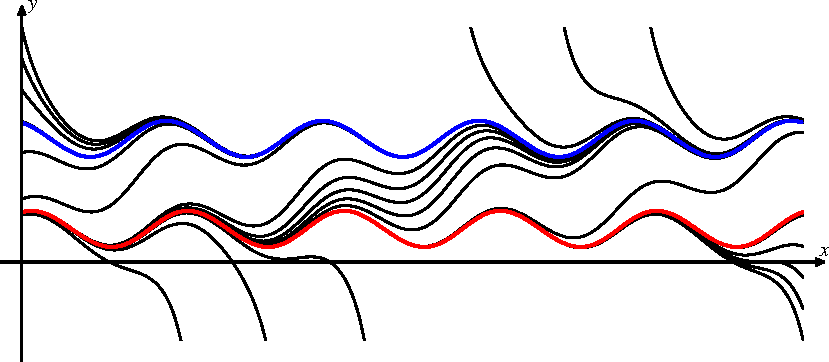
\includegraphics{chapters/images/geometrie-13.pdf}
%\caption{Entwicklung des Systems~(\ref{geometrie:harvest-equation})
%mit $a=5$ und $h=0.8$
%\label{geometrie:harvest-graph}}
%\end{figure}%



\printbibliography[heading=subbibliography]
\end{refsection}

